Ben Trout

2014-12-12

Creo, Testing

\begin{tabular}{|p{5cm}|p{5cm}|}
\hline
Creo&
As we finished testing last week we all decided it would be best to have a plastic ramp. I volunteered to cad and print it up. Making the ramp would be simple enough since we already have a perfect cardboard ramp. I started making the ramp to the same dimensions to the ramp we already had. I CADed up the entire robot up to date and made guides for the ramp.\\
\hline
Testing&
This week as Alex and David finished up wiring by putting all the samantha essentials on the robot we did our first teleop testing wirelessly. We attempted to hook on to the rolling goals, and for the most part it was successful.  
\\
\hline
\end{tabular}

\section*{Creo Ramp}
As I worked on the ramp, I realized how much plastic it would take to print it. I didn’t want to have to print this ramp twice. I had started CADing up the robot at the beginning of the year, but left it off for a while. I decided to finish the entire robot on CAD so I can make sure this ramp will work with our real robot when we print it. Having a virtual robot will allow me to see how parts we need will fit on our actual robot and make sure they’ll work when printed. With the ramp I decided to have the guides actually attached to the ramp and make the ramp wider. I learned how to curv the ends of the guides so they wouldn’t get stuck on the foam in the field as we drove. I made two overhangs on the back of the ramp that go over the back bar. I gave slight room between the overhangs on the ramp and the bar they connect to for correction error. By far the hardest part of the ramp was aligning the holes on the overhang with the bars they are screwed to. The measure tool only does diagonal distance so I had to use the x y coordinates of the holes and transfer those over to the ramp model. 

\section*{Creo Assembly}
For assembling the robot. I downloaded a kit of tetrix parts. I started an assembly in Creo. I learned that you always start with one solid piece as the central piece of the assembly that everything is worked off from. I chose the farthest back bar as the default. This means everything on the x y z plane is measured from this bar. The main assembly tool I use is coincident which means you select two surfaces that will be touching each other, and this is how you align things up. I also learned how to use the distance constraint which allows you to set a distance two surfaces are from each other and CREO will constrain these two at those distances. This was most helpful for axles and also putting a ground touching the wheels. You have to use distance most often with rounded edges like wheels and axles as they have no flat surface to constrain too. The final thing I’ve learned so far is the pin constraint. This allows me to click on our spinner that spins up the ramp and test if it is the right distance from the ramp at all points.

\section*{Testing}
Testing was pretty easy this week. My main goal for this week was to finish the claws that hook onto the ramp and drag it around. We were pressed for time so I just through some lego claws on the axle. We tested at the end of the week, and it was relatively easy to grab the goal, but we’ll definitely have to make the claws out of a harder material to make sure they don’t snap on the field. We also have to make sure that the claws have a finer point to grip the lip of the goals. We also used a continuous rotating servo and we’ll have to switch that to a 180 because the continuous doesn’t stay stiff. 

\begin{center}
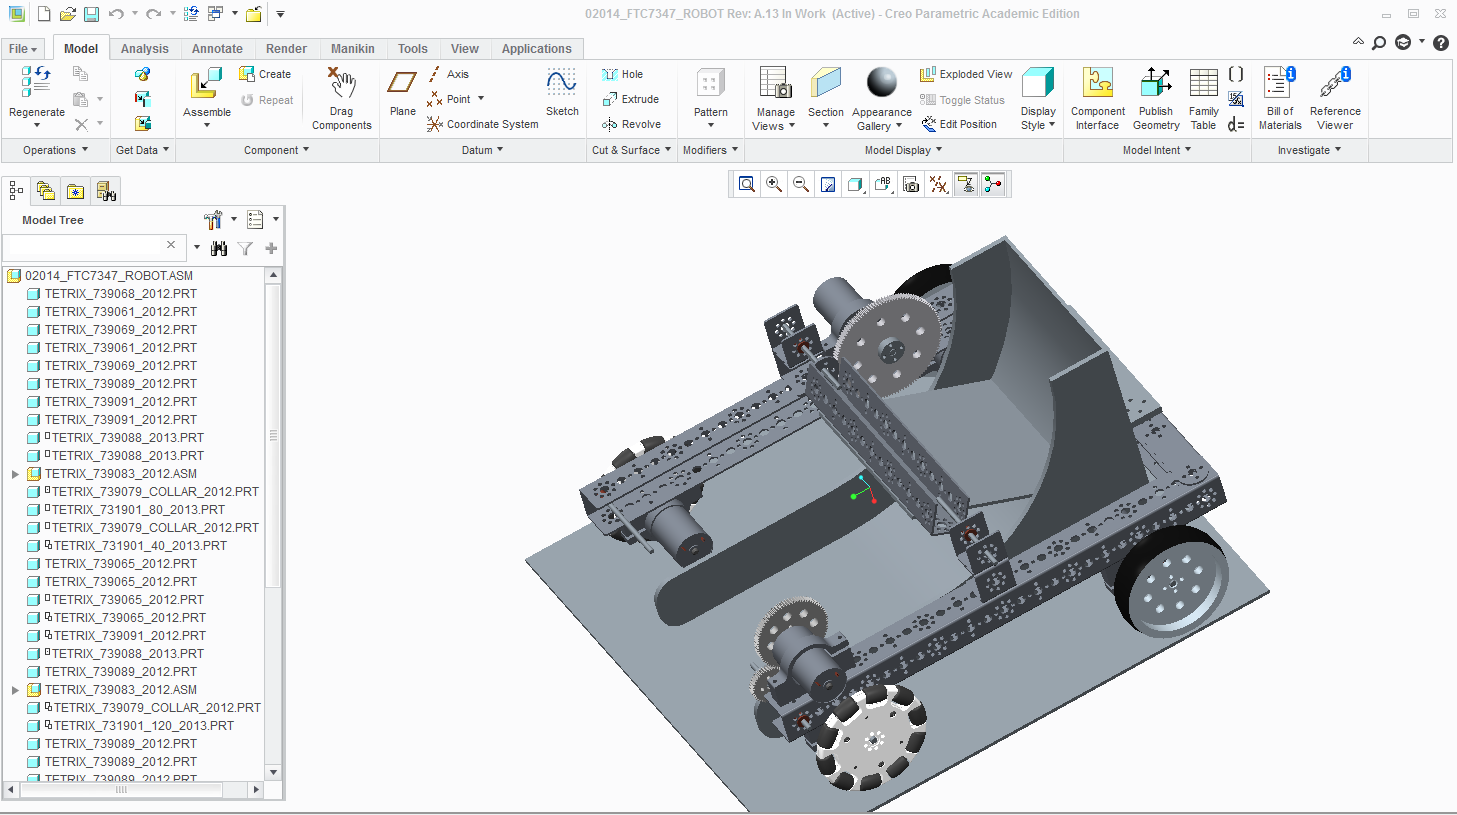
\includegraphics[width=10cm]{./Entries/Images/CreoModelOne.PNG}
\end{center}
